% SPDX-FileCopyrightText: 2023 Jean-Sebastian de Wet, Jan-Philipp Kiel, Pascal Mager
% SPDX-License-Identifier: CC-BY-4.0
%
% LLNCS macro package for Springer Computer Science proceedings Version 2.21 of 2022/01/12
%
\documentclass[runningheads,citeauthoryear]{llncs}
%
\usepackage[T1]{fontenc}
% T1 fonts will be used to generate the final print and online PDFs,
% so please use T1 fonts in your manuscript whenever possible.
% Other font encondings may result in incorrect characters.
%
\usepackage{graphicx}
% Used for displaying a sample figure. If possible, figure files should
% be included in EPS format.
%
% If you use the hyperref package, please uncomment the following two lines
% to display URLs in blue roman font according to Springer's eBook style:
%\usepackage{color}
%\renewcommand\UrlFont{\color{blue}\rmfamily}
%\urlstyle{rm}
%
\usepackage{listings}
\lstset{
  aboveskip=1em,
  breaklines=true,
  captionpos=b,
  escapeinside={\%*}{*)},
  frame=single,
  numbers=left,
  numbersep=1em,
  numberstyle=\tiny,
}
% Used to display Python code.
%
\begin{document}
%
\title{Property-Based Testing of Data Analysis Scripts}
\subtitle{A Focus on Hypothesis for Python}
%\subtitle{Enhancing Reliability in DLR Research}  % Alternative subtitle
%
%\titlerunning{Abbreviated paper title}
% If the paper title is too long for the running head, you can set
% an abbreviated paper title here
%
\author{Jean-Sebastian de Wet \and
  Jan-Philipp Kiel \and
  Pascal Mager}
%
\authorrunning{Group Criterion}
% First names are abbreviated in the running head.
% If there are more than two authors, 'et al.' is used.
%
\institute{University of Cologne, Cologne, Germany}
%
\maketitle              % typeset the header of the contribution
%
\begin{abstract}
  This paper explores property-based testing as a method to ensure data analysis scripts' reliability, especially in German Aerospace Center (DLR) research using Python. It outlines challenges with traditional testing in scenarios with diverse data values, emphasizing the need for innovative testing strategies. The paper thoroughly covers property-based testing, including its history, key principles, use cases, and integration in the test pyramid. It then focuses on Hypothesis for Python, a powerful tool for property-based testing, discussing its use, integration with pytest, and unique features. Real-world application is demonstrated with code examples, highlighting how property-based testing, especially with Hypothesis, strengthens data analysis scripts' reliability. The paper concludes by summarizing key findings and emphasizing the crucial role property-based testing, like Hypothesis, plays in boosting researchers' confidence with unknown data.

  \keywords{Property-Based Testing \and Data Analysis Scripts \and Hypothesis \and Python \and pytest \and Reliability \and Test Pyramid \and Code Examples \and DLR Research.}
\end{abstract}
%
%
%
% [Page 1]
\section{Introduction}
In the evolving landscape of data analysis, the complexity and volume of datasets have grown exponentially~\cite{Taylor2023}, presenting unique challenges across various fields. This surge in data complexity necessitates robust testing methodologies to ensure the accuracy and reliability of data analysis tools and scripts. Traditional testing approaches, primarily based on specific input-output cases, often fall short in addressing the dynamic and unpredictable nature of modern datasets. These limitations are particularly evident in specialized fields like aerospace research, where the data's scope and diversity are exceptionally vast.

The structure of this paper begins with a brief description of the applied methodology, followed by the presentation of results. These results are then discussed in detail, placed in the context of the existing literature and used to derive implications for future works.

% [Page 1-2]
\section{Background}
Within the German Aerospace Center (DLR), the reliability of data analysis scripts is a cornerstone of successful research outcomes. DLR researchers frequently use Python~\cite{Kurnatowski2020}, along with its powerful libraries like pandas\footnote{https://pandas.pydata.org/, accessed: 21.01.2024} and Matplotlib\footnote{https://matplotlib.org/, accessed: 21.01.2024}, for complex data manipulations and visualizations. This introduces significant testing challenges. DLR, being at the forefront of aerospace research and development, deals with an enormous range of data variables, from satellite imagery to flight dynamics.\footnote{https://www.dlr.de/en/dlr/about-us, accessed: 21.01.2024} This variety and complexity of data make testing particularly challenging. This paper explores the adoption of property-based testing, presenting it as an innovative and essential strategy to overcome these testing challenges, especially in scenarios involving large possible value ranges of data.

\section{Method}
Our methodology in tackling these challenges involved two key stages.

\subsection{Literature Study}
The first stage of our methodology involved a thorough literature review on property-based testing. Our objective was to gain an in-depth understanding of its theoretical foundations, including its history, key principles, and diverse applications. The process entailed systematic searches in academic databases and online repositories, using targeted keywords such as "property-based testing" and "automatic test case generation." We focused on selecting literature from various domains, particularly papers highlighting PBT's ability to create diverse test cases. This approach provided a solid knowledge base and included insights on handling complex datasets in DLR. These findings are complemented in the next stage of our study.

\subsection{Prototyping}
The second stage centered on practical application, where we developed a comprehensive guide for using Hypothesis, a property-based testing framework for Python. This guide covered critical aspects including installation, configuration, and integration with Python's pytest\footnote{https://pytest.org/, accessed: 21.01.2024} framework. It also provided practical examples demonstrating the process of defining properties and generating test cases using Hypothesis. To validate our methodology, we conducted a case study that involved applying property-based testing to a data analysis script related to astronauts. This case study served as a real-world application, illustrating the practicality of property-based testing in complex data scenarios.

\section{Results}
First, we uncovered key theoretical insights on property-based testing through our literature study. Then, we demonstrated the practical effectiveness of this approach in our prototype using Hypothesis.

\subsection{Literature Study of Property-Based Testing}
\subsubsection{History}
The origins of property-based testing (PBT) can be traced back more than 20 years ago, even before 2000. While it had already been a subject within information technology research, as seen in Guo (1999) and Fink (1997), it gained significantly more attention with the development of QuickCheck\footnote{https://www.cse.chalmers.se/~rjmh/QuickCheck/, accessed: 21.01.2024}~\cite{Shi2023,Guo1999,Fink1997,MacIver2019,Honarvar2020}. Initially focusing on research questions related to topics such as automation of test input generation and automated techniques in general~\cite{Fink1997} and directing the automated input generator towards values with a higher probability of failure~\cite{Loescher2017}, recent papers have focused on the implementation of different frameworks or platforms and techniques for PBT application~\cite{Padhye2019,Honarvar2020,Shi2023,Corgozinho2023}. To top it off, PBT nowadays enjoys wide-ranging support in different programming languages including automation capabilities~\cite{Chen2022,Padhye2019,Honarvar2020,ElazarMittelman2023,Shi2023}, as well as the application within many different python projects using Hypothesis as a framework for PBT~\cite{Corgozinho2023}.

\subsubsection{Key Concepts}
PBT is a method supporting the formal verification of a software~\cite{Chen2022,Fink1997,Honarvar2020,Paraskevopoulou2015}, focusing on validating high-level or general properties of the software~\cite{Fink1997,Honarvar2020,Corgozinho2023}. Test cases within this method are typically formulated using logical descriptions of the expected behavior of the software~\cite{Chen2022,Fink1997,Honarvar2020,Loescher2017,Corgozinho2023}, including pre- or post-conditions of the system~\cite{Honarvar2020}. To formally validate the system's behavior, a single test case is executed multiple times with randomly generated input to search for counterexamples that violate specific properties or cause a software crash, thereby invalidating said property~\cite{Chen2022,Loescher2017,Padhye2019,ElazarMittelman2023,Paraskevopoulou2015,Corgozinho2023}. Data generators are used for random input generation, which can be adjusted based on a certain domain's needs~\cite{Chen2022,Loescher2017,Padhye2019,ElazarMittelman2023}. Through automated execution of tests with random input, PBT tries to approximate the validity of a property by subjecting it to numerous instantiations within a given input range; otherwise, the property is falsified~\cite{Fink1997,ElazarMittelman2023,Corgozinho2023,Paraskevopoulou2015}. To further elaborate on the properties, which represent the desired behaviour in terms of input and output of given tested functions through specifications~\cite{Chen2022,Fink1997,Loescher2017}, some examples can be given. To start with a simple one, think of a function that adds two numbers (A, B) and returns the sum of both numbers (A + B). You can define a test which asserts that for any given input for either A and B, the function will return the addition of both numbers. Another simple example would be a sort-function. Assume a sort-function sorts a list, the invariant would be, that sorting an already sorted or the same list twice, will result in a sorted and the same list~\cite{Corgozinho2023}. A common example which is frequently used for showcasing PBT are binary search trees~\cite{Corgozinho2023,Shi2023}, where one property to test might be that after "insert[ing] a key into a valid BST, it should maintain its validity"~\cite{Shi2023}. In the context of PBT you would then use logic expressions for your tests and use a random input generator to check whether the given property is violated in any case within a certain input range. It is also possible to apply it to software security concerns such as authentication~\cite{Fink1997} or for verifying the "correctness of hardware [and] external software involved"~\cite{Chen2022}. In summary, PBT allows for the approximation of a system's invariants formal verification~\cite{Fink1997,ElazarMittelman2023,Corgozinho2023}.

\subsubsection{Advantages and Disadvantages}
As previously mentioned, PBT supports the formal validation of software by testing specified properties using randomly generated input for each test. However, describing all expected behavior of a system in a logical style is often less feasible~\cite{Chen2022,Koopman2012}. In contrast, by applying PBT the required endeavour for formal validation can be lowered~\cite{Hritcu2016,Chen2022,Paraskevopoulou2015}. Moreover, specifications used for PBT might also improve cooperation between software engineers and software testers in larger projects, as the language used for defining tests is easier to grasp compared to abstract proofs~\cite{Chen2022,Loescher2017}. Besides this, PBT can also be applied to test in several contexts~\cite{Karlsson2019}, such as interfaces~\cite{Karlsson2019,Francisco2013,LamelaSeijas2013}, e.g. by testing invariants regarding the responses of requested URLs of REST-APIs~\cite{Karlsson2019}. Other potential domains of application include telecom systems~\cite{Arts2006}, file synchronisation services~\cite{Hughes2016} and databases~\cite{Arts2015}. Despite its wide applicability and advantages in formal validation, PBT reduces engineering effort in terms of defining individual test cases and input parameters~\cite{Chen2022,Loescher2017,Corgozinho2023} and may also incentivize SEs to design code that can be easily expressed by properties~\cite{Chen2022}. More specifically, when compared to manually written tests like in unit-testing, PBT allows the software engineer to put more emphasis on ensuring and restoring correctness of the software and less on "defining test case inputs, examples, and scenarios"~\cite{Corgozinho2023}, turning it into a much less "mundane"~\cite{Loescher2017} effort. It therefore reduces costs related to testing, including costs induced by changes made to the software~\cite{Chen2022,Loescher2017}. Furthermore it allows for validating a software based on a much larger range of inputs~\cite{Loescher2017} [Hypothesis for Software Testing Research] and even more creative or sophisticated inputs~\cite{Arts2015}. Therefore PBT complements traditional testing techniques by unveiling yet unknown bugs within even well tested systems~\cite{Arts2015,Hughes2016,Arts2006} and in general, is useful for finding bugs within the implementation of a software and its specifications~\cite{Chen2022,Fink1997,Loescher2017,Paraskevopoulou2015,Claessen2000,Corgozinho2023}.

Although PBT offers quite some advantages, it does not come without any disadvantages. Due to the randomness of the input generator provided by tools, the chances of finding more specific bugs is reduced, depending on the portion of erroneous inputs of the entire input range, thus potentially failing to unveil errors~\cite{Loescher2017,Padhye2019,ElazarMittelman2023,Shi2023}. It should be noted that processing a large number of tests can lead to reduced efficiency~\cite{ElazarMittelman2023,Shi2023}, as it involves attempting to approximate a formal proof using numerous randomly selected scenarios~\cite{Fink1997,ElazarMittelman2023,Paraskevopoulou2015}. Löscher (2017) gave quite a good fictional example using a "system of network nodes"~\cite{Loescher2017}. They tried to falsify the property that for any input scenarios (graphs created), the longest of the shortest paths "between the sink and other nodes [...] should not exceed 21 hops"~\cite{Loescher2017}. Even after "100000 tests"~\cite{Loescher2017} they were not able to falsify the property, which could be done "by hand"~\cite{Loescher2017}. A possible solution to this problem is implied by the usage of individually conceptualised data generators~\cite{Loescher2017,ElazarMittelman2023,Shi2023,Paraskevopoulou2015,Claessen2000} or targeted property-based testing~\cite{Loescher2017}. While constraining data generators in order to cancel a test by using pre-conditions as a form of domain knowledge represents an option to reduce computation effort~\cite{Loescher2017,ElazarMittelman2023,Shi2023}, targeted property-based testing achieves this by guiding the input generator~\cite{Loescher2017}. The idea is to increase the chance of generating inputs causing the violation of a property, by applying "search techniques"~\cite{Loescher2017}. However, the first technique of implementing specified data generators comes with its own challenges regarding the development~\cite{Loescher2017,ElazarMittelman2023,Shi2023}, resulting in a reduced attractiveness of PBT.

\subsubsection{Classification within the Test Pyramid}
In order to classify PBT within the test pyramid, we focus on the level of unit and integration (service) testing~\cite{Aniche2022,Radziwill2020}. Current literature indicates that PBT has not yet been applied for testing at the highest level of either system or UI tests~\cite{Radziwill2020,Aniche2022}, making them irrelevant for our analysis.

\begin{figure}
  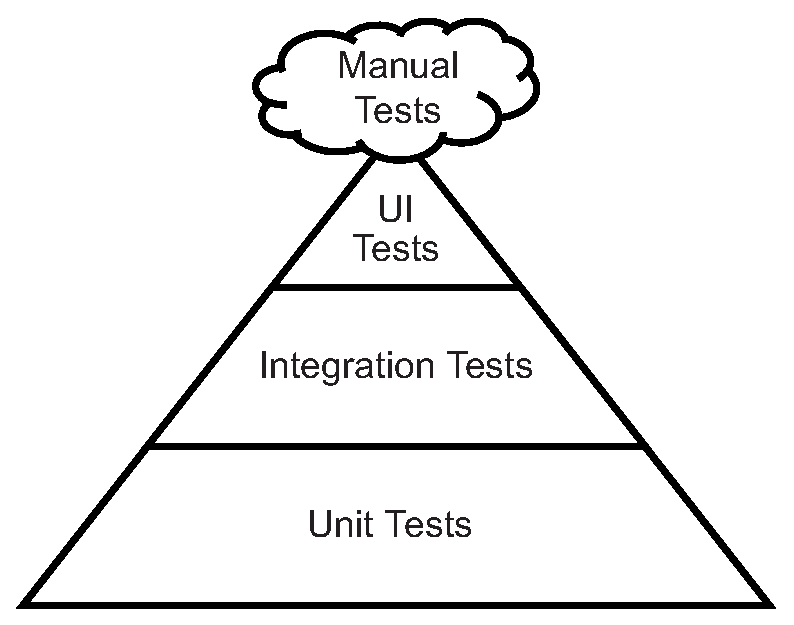
\includegraphics[width=.5\textwidth]{includes/test_pyramid.eps}
  \caption{Test Pyramid. Based on Vocke, H.: The Practical Test Pyramid (2018). https://martinfowler.com/articles/practical-test-pyramid.html}
  \label{fig:test_pyramid}
\end{figure}

Beginning with unit testing, "developers perform unit testing to ensure that each component correctly implements its design and is ready to be integrated into a system of components"~\cite{Hartmann2000}. In other words, each function or module of a system is tested in an isolated manner. Furthermore it emphasized on "example-based"~\cite{Corgozinho2023} testing individual - also referred to as the "smallest parts"~\cite{Aniche2022} - of a system ~\cite{Hartmann2000,Corgozinho2023}.

Within integration tests, as the name suggests, every component of a system is integrated with each other, including relevant external components~\cite{Aniche2022,Hartmann2000,Radziwill2020}. The goal is to ensure that interaction between the given components works correctly and therefore, the combined set of functionality~\cite{Hartmann2000,Aniche2022}.

Although the majority of the use cases explaining how PBT works focus on individual components, such as functions for adding numbers, inserting nodes in binary search trees,
and managing sorted lists, it also offers potential applications concerning the physical and external aspects of software~\cite{Chen2022}. Referring back to the example regarding authentication, one can test not only the authentication functionality of a system but also the integration of its respective authentication services~\cite{Fink1997}. Additionally, PBT has been utilized in various scenarios such as testing RESTful APIs within the context of OpenAPIs~\cite{Karlsson2019}, telecom systems~\cite{Arts2006}, synchronisation services~\cite{Hughes2016} or AUTOSAR software~\cite{Arts2015}. For instance, in the case of QuickREST, response codes can be used to differentiate between invalid and URL requests, ultimately revealing previously unknown "underspecification" in the utilized OpenAPI documentation~\cite{Karlsson2019}. Similarly, in the context of AUTOSAR, testing correct request processing unveiled a previously unknown bug related to task prioritization~\cite{Arts2015}. Lastly, complete crashes of addressed components can also be observed~\cite{Arts2006}.

Consequently, the PBT method can be applied to both unit and integration testing. In practical terms, PBT is commonly employed for unit testing and is well-suited for this purpose, as its highlighted advantages demonstrate complementary effects compared to simple example-based unit testing. However, its applicability is not restricted solely to unit testing. Existing literature has shown that it also extends to testing the integration of various components.

\subsubsection{Tools and Programming Languages}
As previously mentioned, PBT is widely supported across various programming languages~\cite{Chen2022,Shi2023}. It is supported by Java (Quicktheories\footnote{https://github.com/quicktheories/QuickTheories, accessed: 21.01.2024}), coq (QuickChick\footnote{https://github.com/QuickChick/QuickChick, accessed: 21.01.2024}), Scala (ScalaCheck\footnote{https://scalacheck.org/, accessed: 21.01.2024}), Erlang (QuickCheck\footnote{http://www.quviq.com/products/erlang-quickcheck/, accessed: 21.01.2024} and PropEr\footnote{https://proper-testing.github.io/, accessed: 21.01.2024}), Haskell (QuickCheck\footnote{https://hackage.haskell.org/package/QuickCheck, accessed: 21.01.2024}), OCaml (QCheck\footnote{https://github.com/c-cube/qcheck/, accessed: 21.01.2024} and Crowbar\footnote{https://github.com/stedolan/crowbar, accessed: 21.01.2024}) to name a few examples~\cite{MacIver2016,Padhye2019,Paraskevopoulou2015,Arts2008,Papadakis2011,Claessen2000}. Obviously many of these were inspired by QuickCheck, being the tool popularising PBT. However, this study focuses on Hypothesis\footnote{https://hypothesis.works/, accessed: 21.01.2024}, a Python-based PBT implementation framework. This framework has garnered significant attention recently~\cite{Corgozinho2023,MacIver2019}, is compatible with pytest, unittest\footnote{https://docs.python.org/3/library/unittest.html, accessed: 21.01.2024} and "probably many others", as well as being open source "under the Mozilla Public License 2.0"\footnote{https://hypothesis.works/products/, accessed: 21.01.2024}.

% [Pages 5-9]
\subsection{Prototype of Data Analysis Scripts using Hypothesis for Python}
\subsubsection{Overview}
Hypothesis is a Python library for Property-Based Testing. The focus is on having a simple manner in which software can be tested. The main difference when writing test cases in Hypothesis, versus traditional unit tests, is that instead of giving concrete input, performing the function, and asserting something about the result, the focus is on trying to make the assertions hold for all data matching a certain specification.

The advantages are that Hypothesis helps to discover edge cases and hidden bugs which were not thought of during typical testing. It also helps to make the tests more robust, seeing as a wide variety of inputs, some even random, are used.
Furthermore, it can help save time, by encompassing many traditional unit test cases into one PBT test case. And lastly, Hypothesis also integrates into other testing frameworks such as pytest and nose. In terms of disadvantages, Hypothesis might lead to longer execution times of test suites. This is due to a Hypothesis test case generating many more subordinate test cases and running them. Although Hypothesis tries to reproduce the input that caused the test case to fail, this might not always work and it can therefore sometimes be challenging to understand why a test case failed.
Lastly, one typically has less control when using PBT in comparison to a typical unit test.\footnote{https://hypothesis.readthedocs.io/en/hypothesis-python-4.57.1/, accessed: 10.01.2024}. The majority of these advantages and disadvantages correspond with the general advantages and disadvantages of PBT that can be found within the academic literature.

\subsubsection{Strategies and Data Generation}
One of the main concepts of Hypothesis is the idea of search strategies. Search strategies refer to how hypothesis will try to generate input for the test function. Or rather, what it will use to "search" for bugs. Hypothesis has plenty of different search strategies that can be used. For instance, it can generate text, floats, integers, boolean values, a value of a given set of values and values that match a given regex. Furthermore, these search strategies can be refined by input parameters. This can, for instance, limit the size of the floats generated or allow only dates between date ranges.

The format of using a search strategy in Hypothesis is consistent. Typically, an object representing a search strategy is instantiated using the syntax \texttt{st.(type)}, where \texttt{type} is the specific search strategy to use (e.g., \texttt{text}, \texttt{float}, \texttt{date}). The instantiation can be further refined by specifying parameters. The parameters can for instance, limit the dates to a certain range or only generate floats up to a certain size. By default, Hypothesis will try to create 100 different tests

\subsubsection{Hypothesis Usage}
In order to use Hypothesis, one first needs to install the Hypothesis package. This can be done by using the command \texttt{pip install hypothesis}. The specific setup used is as follows:

\begin{itemize}
  \item Operating System: Ubuntu 22.04.3 LTS
  \item Python Version: 3.10.12
  \item pip Version: 22.0.2
  \item hypothesis Version: 6.92.2
\end{itemize}
However, Hypothesis officially tries to support the latest version of Python.\footnote{https://hypothesis.readthedocs.io/en/latest/, accessed: 10.01.2024}

\vspace{5mm}
\noindent Consider the following code snippet:
\begin{lstlisting}[language=Python]
  from hypothesis import given
  import hypothesis.strategies as st
  
  @given(st.integers())
  def test_builtin_abs(x: int) -> None:
      assert abs(x) >= 0
      assert abs(x) == (x if x >= 0 else -x)
\end{lstlisting}
The main way in which the Hypothesis test is annotated, is using the \texttt{given} decorator. The \texttt{given} decorator takes a search strategy object and uses this to populate the parameters of the function. In this case, integers are generated to be used as input to the $x$ parameter of the function.

This function then asserts that certain properties hold for each value of $x$ generated. In this example, it tests that the built-in absolute value function of Hypothesis works as it is intended to work.

\vspace{5mm}
\noindent Another key aspect of Hypothesis is being able to create new, unique search strategies. The following code block is an example of this:

\begin{lstlisting}[language=Python,caption={Complex Input Example from code/tutorial.ipynb}]
  from hypothesis.strategies import composite

  PI = 3.14159
  
  @composite
  def custom_input_generator(draw) -> tuple[float, str]:
      decimal = draw(st.floats(max_value=PI))
      text = draw(
        st.text(alphabet=st.characters
        (whitelist_categories=['Lu']), 
      min_size=2, max_size=5))
      return decimal, text
  
  @given(custom_input_generator())
  def test_custom_input_generator
          (generated_input: tuple[float, str]) -> None:
      decimal, text = generated_input
      assert decimal <= PI
      assert len(text) >= 2 and len(text) <= 5
      assert text.isupper()
\end{lstlisting}
The \texttt{composite} decorator is used to specify a function that generates a custom search strategy. The function works by combining existing search strategies. So in the above, the float search strategy is used to generate floats up until a max value of PI. Then, the text search strategy is used to generate text that consists of only upper-case letters and is between 2 and 5 characters long. The test function simply tests that the search strategy generation function generates output of the correct form.

\subsubsection{Integration with pytest}
The integration with pytest is automatic. It is sufficient to run pytest in the traditional sense, as pytest will automatically pick up the hypothesis-tests.

\subsubsection{Changing number of test cases generated}
The number of test cases that are generated can be changed with the following decorator:

\begin{lstlisting}[language=Python]
from hypothesis import settings

@given(st.integers())
@settings(max_examples=100)
def test_builtin_abs(x: int) -> None:
  ...
\end{lstlisting}

\noindent Globally this can be done as follows:
\begin{lstlisting}[language=Python]
  settings.register_profile("default", max_examples=100)
  settings.load_profile("default")
\end{lstlisting}

% [Pages 9-13]
\subsubsection{Application for Data Analysis Scripts}
Hypothesis can be used to test data analysis scripts. In particular, Hypothesis can be helpful to ensure that the data preparation and data cleaning steps are properly tested. This is due to Hypothesis being able to simulate a wide range of inputs, which can then be used to ensure that the functions are robust. The Data Analysis script that Hypothesis will be applied to, is a script that was provided by the DLR \cite{Stoffers2021Astronaut}.

\vspace{5mm}
\noindent The first function that will be examined is the \texttt{calculate\symbol{95}age} function:

\begin{lstlisting}[language=Python]
  def calculate_age(born):
    today = date.today()
    return today.year - born.year - 
      ((today.month, today.day) < (born.month, born.day))
\end{lstlisting}
This is an auxiliary function in the data preparation script. It takes a date object and calculates the current age by considering the time that has passed since the given date. This function can be tested as follows:

\begin{lstlisting}[language=Python]
@given(st.dates(min_value=date(1920, 1, 1), 
                    max_value=date.today()))
def test_calculate_age(born: date) -> None:
  age = calculate_age(born)
  assert age >= 0 and 
  age <= (born.today().year - born.year)
\end{lstlisting}
The test generates random dates between the 1st of January 1920 and the current date. It then confirms that the \texttt{calculate\symbol{95}age} function works as intended.

\vspace{5mm}
\noindent The next function that will be tested is arguably the most important function in the script, the function that is used to prepare the data sets:

\begin{lstlisting}[language=Python]
def prepare_data_set(df):
  df = rename_columns(df)
  df = df.set_index("astronaut_id")

  # Set pandas dtypes for columns with date or time
  df = df.dropna(subset=["time_in_space"])
  df["time_in_space"] = df["time_in_space"].astype(int)
  df["time_in_space"] = pd.to_timedelta
  (df["time_in_space"], unit="m")
  df["birthdate"] = pd.to_datetime(df["birthdate"])
  df["date_of_death"] = pd.to_datetime
  (df["date_of_death"])
  df.sort_values("birthdate", inplace=True)

  # Calculate extra columns from the original data
  df["time_in_space_D"] = df["time_in_space"] 
  / pd.Timedelta(days=1) # df["time_in_space_D"] = 
  df["time_in_space"].astype("timedelta64[D]")
  df["alive"] = df["date_of_death"].apply(is_alive)
  df["age"] = df["birthdate"].apply(calculate_age)
  df["died_with_age"] = df.apply(died_with_age, axis=1)
\end{lstlisting}

\vspace{5mm}
\noindent Please note that the line:
\begin{lstlisting}[language=Python]
  df["time_in_space_D"] = df["time_in_space"].astype("timedelta64[D]")
\end{lstlisting}
from the original script has been altered to:
\begin{lstlisting}[language=Python]
  df["time_in_space"] / pd.Timedelta(days=1)
\end{lstlisting}
in the revised version.
\vspace{5mm}

\noindent Hypothesis is well-suited to test even a complicated function like the above function. The focus will be on generating appropriate inputs to the \texttt{prepare\symbol{95}data\symbol{95}set} function:

\begin{lstlisting}[language=Python]
  @st.composite
  def astronaut_data(draw) -> dict:
      astronaut = draw(st.from_regex(
        r"http://www\.wikidata\.org/entity/Q\d+",
         fullmatch=True))
      astronautLabel = draw(
        st.from_regex(r"[A-Z][a-z]+ [A-Z][a-z]+"
        , fullmatch=True))
      birthdate = draw(
        st.dates(min_value=date(1920, 1, 1), 
                 max_value=date(2030, 12, 31)))
      birthplaceLabel = draw(
        st.from_regex(r"[A-Z][a-z]+", fullmatch=True))
      sex_or_genderLabel = draw(
        st.sampled_from(["male", "female"]))
      time_in_space = draw(
        st.integers(min_value=1, max_value=900)) 
      date_of_death = draw(st.one_of(
          st.none(), 
          st.dates(birthdate + timedelta(days=1), 
                   max_value=date(2030, 12, 31))
          )
      )
  
      birthdate_str = birthdate.strftime(
        "%Y-%m-%dT00:00:00Z")
      date_of_death_str = date_of_death.strftime(
        "%Y-%m-%dT00:00:00Z") if date_of_death else None
  
    ...
\end{lstlisting}
This function generates a wide variety of inputs. Specifically, it generates an astronaut link and label using regex search strategies. It then generates a birthdate that falls within a certain range, using the \texttt{st.dates} strategy as well as by specifiying a min and max value. The sex or gender label is then generated using \texttt{st.sampled} from which then allows Hypothesis to generate input using the values male and "female". The time in space is then generated using \texttt{st.integers()} and constraint to a given range. Then the date of death is used by combining two strategies, \texttt{st.none} and \texttt{st.dates}, of which one will be selected. The birthdate and if present death date, are then transformed into the corresponding format that the data preparation script expects.

This shows how Hypothesis can be used to generate complex inputs which can then be used to test data analysis scripts. This will result in the following output.
\subsubsection{Discovering Issues}
Hypothesis can also be very helpful in finding potential bugs and making data analysis scripts more robust. In particular, by removing the max value of the time in space strategy, Hypothesis will trigger the data analysis script to crash. The following output is returned by Hypothesis:

\begin{verbatim}
OverflowError: Python int too large to convert to C long
Falsifying example: test_prepare_data_set(
    data=[{'astronaut': 'http://www.wikidata.org/entity/Q0',
      'astronautLabel': 'Aa Aa',
      'birthdate': '2000-01-01T00:00:00Z',
      'birthplaceLabel': 'Aa',
      'sex_or_genderLabel': 'male',
      'time_in_space': 18446744073709551616,
      'date_of_death': '2000-01-02T00:00:00Z'}],
  )
\end{verbatim}

\noindent The specific can be traced back to :

\begin{lstlisting}[language=Python]
  [...]
  df = rename_columns(df)
  df = df.set_index("astronaut_id")

  # Set pandas dtypes for columns with date or time
  df = df.dropna(subset=["time_in_space"])
  df["time_in_space"] = df["time_in_space"]
  .astype(int) # This caused line caused the error
  df["time_in_space"] = pd.to_timedelta
  (df["time_in_space"], unit="m")
  df["birthdate"] = pd.to_datetime(df["birthdate"])
  df["date_of_death"] = pd.to_datetime
  (df["date_of_death"])
  df.sort_values("birthdate", inplace=True)
  [...]
\end{lstlisting}
And it is due to a Python integer being to large to be converted to a C long. The data preparation script can therefore be improved, by checking beforehand that the integers are within a specified range.

\vspace{5mm}
\noindent As for another example, by removing the max date range, the following error will be produced:

\begin{verbatim}
pandas._libs.tslibs.np_datetime.OutOfBoundsDatetime: 
Out of bounds nanosecond timestamp: 2263-01-01T00:00:00Z, 
at position 0
Falsifying example: test_prepare_data_set(
    data=[{'astronaut': 'http://www.wikidata.org/entity/Q0',
      'astronautLabel': 'Aa Aa',
      'birthdate': '2000-01-01T00:00:00Z',
      'birthplaceLabel': 'Aa',
      'sex_or_genderLabel': 'male',
      'time_in_space': 1,
      'date_of_death': '2263-01-01T00:00:00Z'}],) 
\end{verbatim}

\vspace{5mm}
\noindent The \texttt{datetime64[ns]} data type in pandas/NumPy is limited to the range of dates from 1677-09-21 to 2262-04-11 because it stores dates as 64-bit integers representing nanoseconds since the Unix epoch (January 1, 1970). Therefore, if NumPy tries to convert the date of death, \texttt{'2263-01-01T00:00:00Z'}, the script will crash. This shows yet another example of how the data script can be made more robust. Specifically, by checking that the dates are within range that pandas/NumPy can process.

\section{Discussion}

% [Page 13-14]
\section{Conclusion}
\begin{itemize}
  \item Summarize the key points discussed in the paper.
  \item Emphasize the importance of property-based testing, particularly with tools like Hypothesis, in enhancing the reliability of data analysis scripts.
\end{itemize}
%
% ---- Bibliography ----
%
% BibTeX users should specify bibliography style 'splncs04'.
% References will then be sorted and formatted in the correct style.
%
\bibliographystyle{splncs04}
\bibliography{references}
\end{document}
